\phantomsection
\section*{二、LLM 推理基础、问题空间与优化分类}
\addcontentsline{toc}{section}{二、LLM 推理基础、问题空间与优化分类}

\phantomsection
\subsection*{2.1 LLM 推理的基本执行机制}
\addcontentsline{toc}{subsection}{2.1 LLM 推理的基本执行机制}

本文关注的 LLM 推理以在线生成服务为主：系统接收输入上下文，并以自回归方式逐 token 生成输出。与输入输出形状较固定的传统 DNN 推理相比，LLM 请求的输入长度、输出长度和到达时间持续变化，decode 还依赖已经生成的 token 和 KV Cache。随着上下文与生成长度增加，KV Cache 也会增长，因此系统需要同时控制吞吐、时延、显存占用和服务质量。

图~\ref{fig:llm-serving-workflow} 给出了典型服务流程。上层 serving policy 负责请求准入、路由、排队和执行顺序；batching/scheduling 模块根据服务目标、请求优先级、长度、实例负载和 KV 容量，调整等待窗口、token 上限、prefill/decode 资源配额以及当前参与执行的请求集合。该集合既可包含尚未处理完输入上下文的 prefill 请求，也可包含正在逐 token 生成的 decode 请求。底层 inference runtime 完成模型计算和 KV 管理，并把 TTFT、TPOT、ITL、队列长度和 KV 使用量反馈给控制模块，用于下一轮调度。

\begin{figure}[htbp]
    \centering
    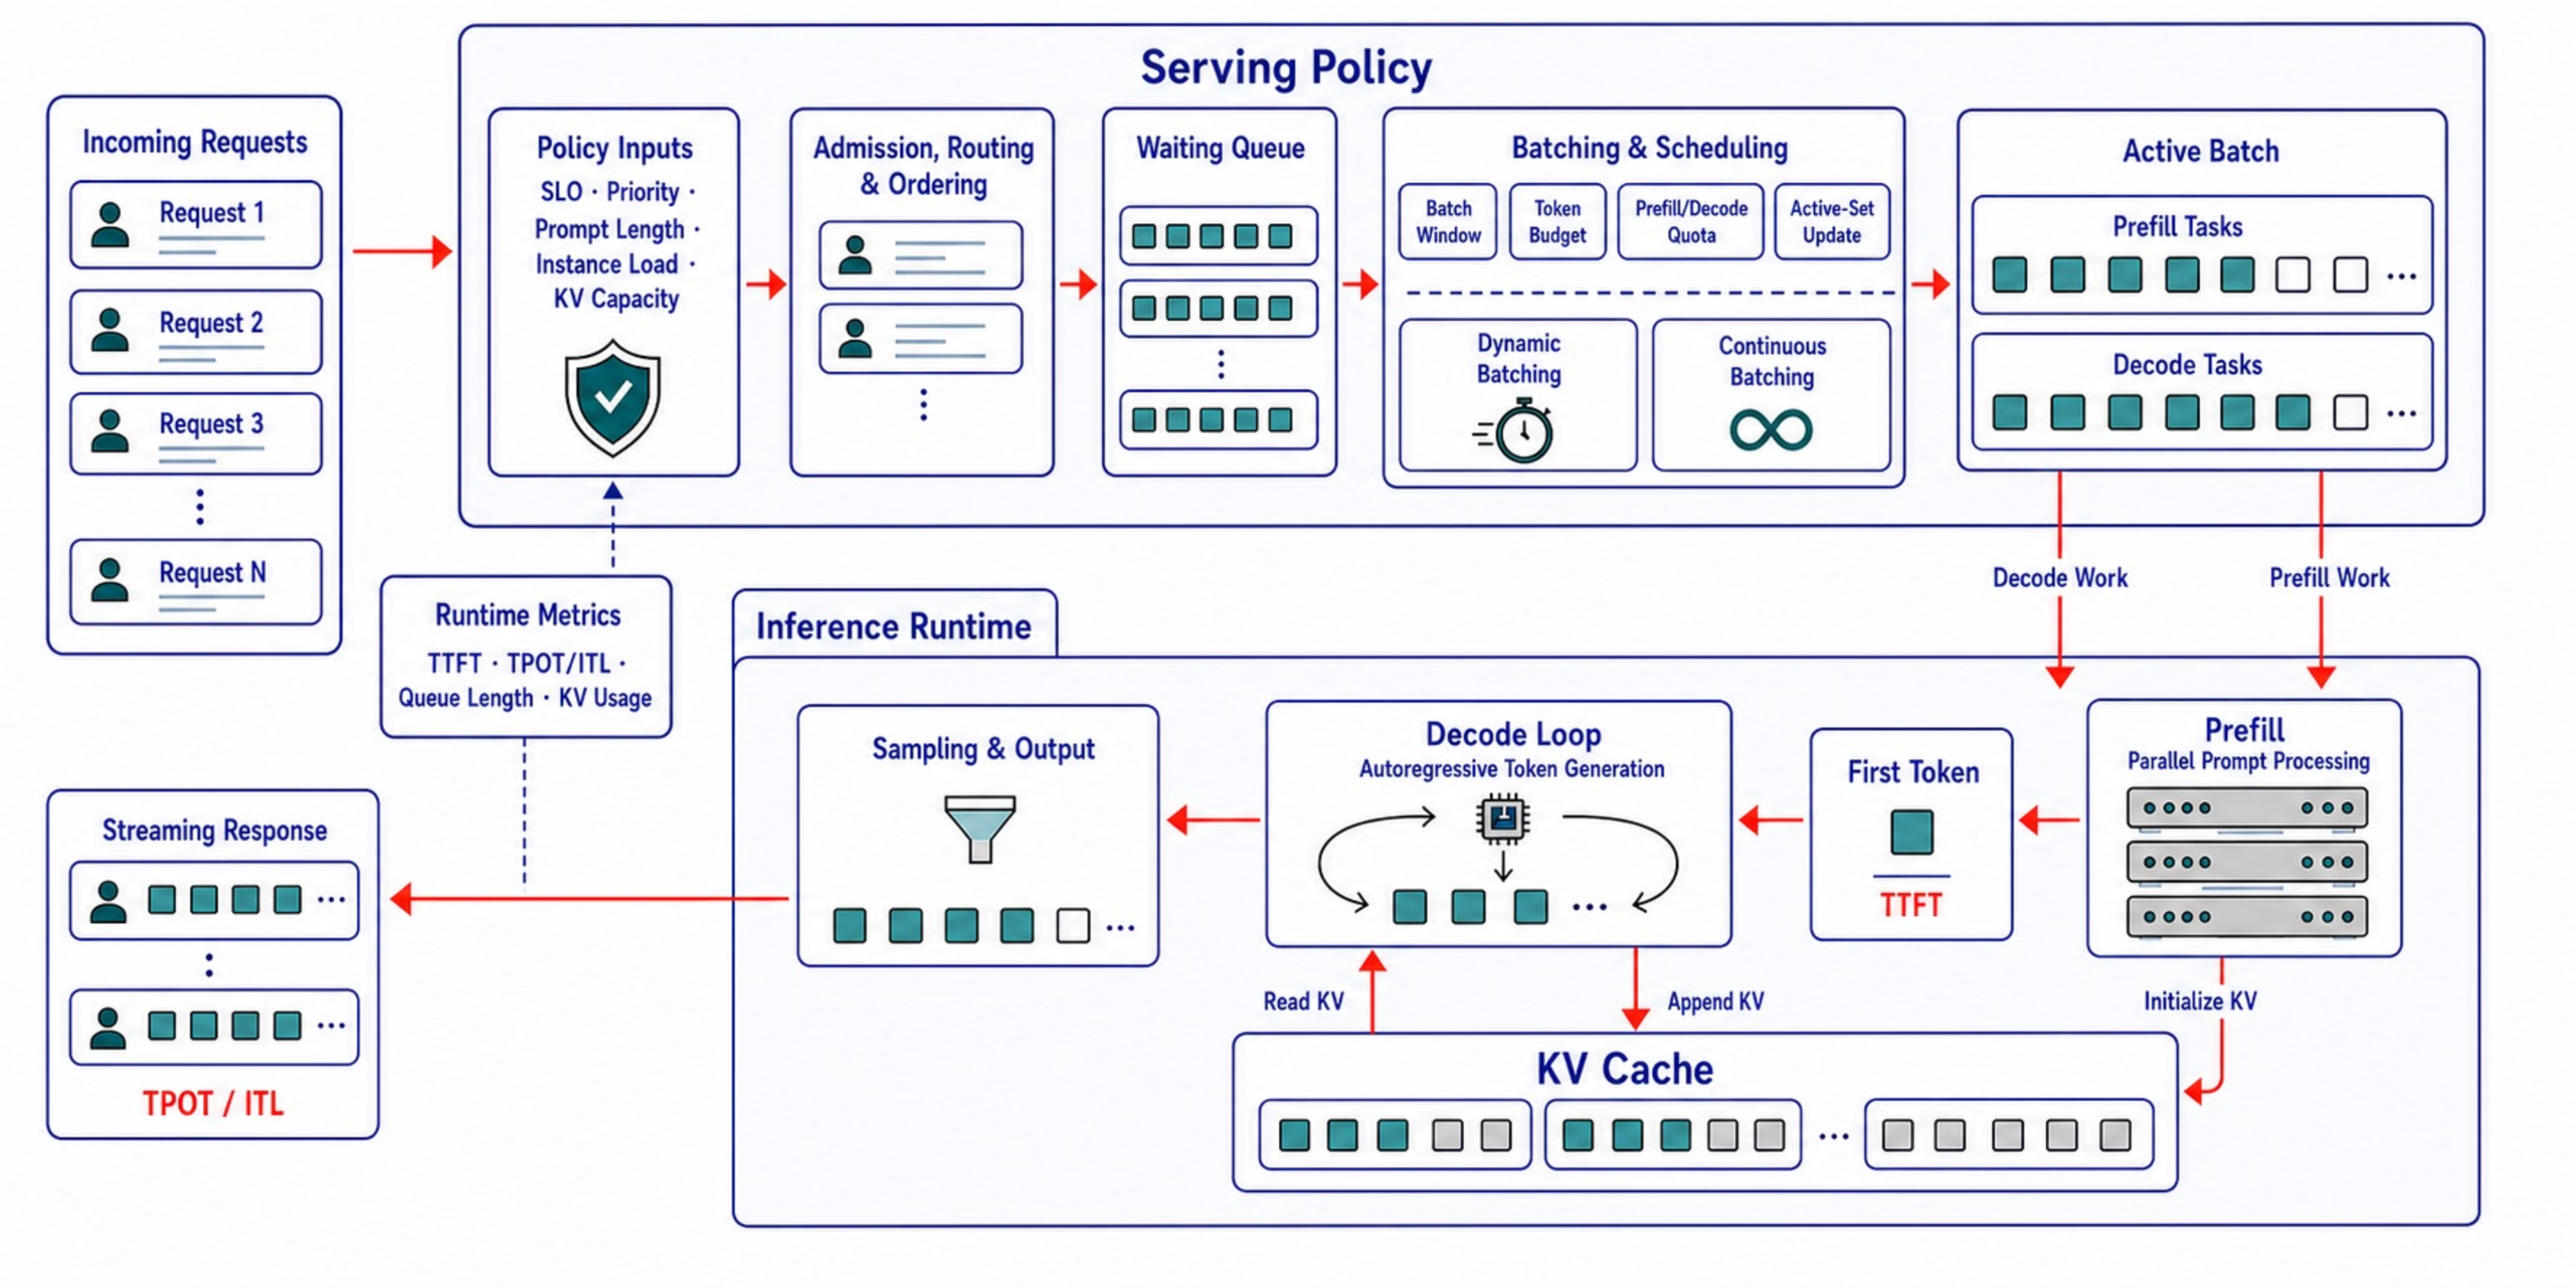
\includegraphics[width=\textwidth]{figures/ch2_llm_serving_workflow.pdf}
    \caption{\textbf{LLM serving 基础服务流程。}Serving policy 作为上层控制面，内部包含准入、路由、排序、请求队列和 batching/scheduling，并根据业务与运行状态形成同时包含 prefill tasks 与 decode tasks 的活动批次；inference runtime 分别执行 Prefill、KV Cache 管理和逐 token Decode，最终形成流式响应并将运行指标反馈给 serving policy。}
    \label{fig:llm-serving-workflow}
\end{figure}

\phantomsection
\subsubsection*{2.1.1 Prefill 与 Decode}
\addcontentsline{toc}{subsubsection}{2.1.1 Prefill 与 Decode}

当今主流的大模型是基于decoder架构的。对于 decoder-only 自回归大模型，一次请求通常分为 \textbf{Prefill} 和 \textbf{Decode} 两个阶段。


\textbf{Prefill 阶段}负责处理完整输入上下文，包括用户 prompt、历史对话、系统提示词和检索增强内容等。模型对整段上下文并行计算 attention 和 FFN，为每一层生成后续 decode 复用的初始 KV Cache，并根据最后位置的输出分布产生首个输出 token。该阶段矩阵规模较大、并行度较高，通常更受计算能力限制，主要影响 TTFT，即 Time To First Token。


\textbf{Decode 阶段}负责逐 token 生成输出。每一步 decode 输入上一步生成的新 token，同时读取历史 KV Cache，计算当前 token 的 attention 和 FFN，并将新增 KV 写回缓存。该阶段每步计算粒度较小、状态依赖强、访存频繁，通常更受显存带宽和单步时延限制，主要影响 TPOT、ITL 和持续生成吞吐。


Prefill 和 Decode 的资源特征差异直接影响 LLM serving 的系统设计。Prefill 以大规模矩阵计算为主，Decode 则由高频、小粒度并且依赖历史状态的迭代组成。因此，推理系统通常分别考虑两个阶段的 batching、调度、KV 管理和分布式执行方式。




\phantomsection
\subsubsection*{2.1.2 KV Cache}
\addcontentsline{toc}{subsubsection}{2.1.2 KV Cache}

KV Cache 是 LLM decode 阶段最核心的运行时状态。自回归生成中，第 t 个 token 的 attention 需要访问前面所有 token 的 key/value。如果每一步都重新计算历史 token 的 key/value，会产生大量重复计算。KV Cache 的作用是在 prefill 阶段保存历史 token 的 key/value，在 decode 阶段复用这些历史 KV，只为新 token 计算新增 KV。


KV Cache 降低了 decode 阶段的重复计算，但也引入了显著的内存状态问题。KV 占用会随 batch size、上下文长度、输出长度、模型层数和 KV head 数增长。在长上下文、多轮对话和高并发场景中，KV Cache 往往成为显存容量和显存带宽的重要瓶颈。vLLM 的 PagedAttention~\cite{kwon2023efficient}、vAttention~\cite{prabhu2025vattention} 的动态 KV 内存管理和 Mooncake~\cite{qin2025mooncake} 的 KVCache-centric serving，分别从分页分配、动态地址映射和分布式 KV 存储等角度降低状态管理开销；相关综述进一步覆盖缓存淘汰、卸载、量化和持久化等方向 \cite{zhou2024survey,pan2025survey}。


典型 KV 相关优化如表~\ref{tab:kv-cache-optimizations} 所示：


\begin{table}[!htbp]
    \centering
    \caption{\textbf{典型 KV Cache 相关优化及作用}}
    \label{tab:kv-cache-optimizations}
    \renewcommand{\arraystretch}{1.45}
    \scriptsize
    \setlength{\tabcolsep}{4pt}
    \begin{tabularx}{\textwidth}{@{}>{\hsize=0.55\hsize\raggedright\arraybackslash}X >{\hsize=1.45\hsize\raggedright\arraybackslash}X@{}}
        \toprule
        \textbf{方向} & \textbf{作用} \\
        \midrule
        PagedAttention / memory paging & 降低 KV 分配碎片，提高显存利用率 \\
        \tabrowrule
        Prefix cache / RadixAttention & 复用共享前缀，减少重复 prefill \\
        \tabrowrule
        KV compression / quantization & 降低 KV 存储和传输成本 \\
        \tabrowrule
        KV eviction & 在显存不足时淘汰低价值 KV \\
        \tabrowrule
        KV offloading & 将部分 KV 放到 CPU、本地存储、远端内存或其他节点 \\
        \tabrowrule
        Distributed KV cache & 在多 worker / 多节点场景下管理 KV 状态分布 \\
        \bottomrule
    \end{tabularx}
\end{table}




\phantomsection
\subsubsection*{2.1.3 Batching 与 Scheduling}
\addcontentsline{toc}{subsubsection}{2.1.3 Batching 与 Scheduling}

Batching 是 LLM serving 提高硬件利用率和吞吐量的主要机制。单个请求在 decode 阶段的每步计算粒度较小，只服务少量请求时加速器容易出现计算单元空闲。Batching 通过合并多个请求扩大矩阵运算规模，提高 GPU/NPU 的并行执行效率，并分摊算子启动和调度等固定开销。


LLM batching 与传统 DNN batching 的执行条件不同。传统推理服务中的动态批处理器通常在请求执行前按等待窗口和 batch size 形成批次 \cite{nvidia2026triton}；LLM 请求的输入长度、到达时间和输出长度差异较大，decode 请求会逐步完成并释放 batch slot，长 prompt 的 prefill 还可能阻塞短请求的 decode。因此，现代 LLM serving 系统通常结合 dynamic batching、continuous batching、iteration-level scheduling 和 chunked prefill。Orca~\cite{yu2022orca} 代表迭代级调度路线，Sarathi-Serve~\cite{agrawal2024taming} 代表 chunked prefill 路线；近期综述也将 batching/scheduling 与算子优化、内存管理并列为 LLM 推理系统的主要组成部分 \cite{zhou2024survey,zhen2025taming,pan2025survey}。


典型调度机制如表~\ref{tab:serving-scheduling-mechanisms} 所示：


\begin{table}[!htbp]
    \centering
    \caption{\textbf{典型 LLM Serving 调度机制及作用}}
    \label{tab:serving-scheduling-mechanisms}
    \renewcommand{\arraystretch}{1.45}
    \scriptsize
    \setlength{\tabcolsep}{4pt}
    \begin{tabularx}{\textwidth}{@{}>{\hsize=0.55\hsize\raggedright\arraybackslash}X >{\hsize=1.45\hsize\raggedright\arraybackslash}X@{}}
        \toprule
        \textbf{机制} & \textbf{作用} \\
        \midrule
        Dynamic batching & 根据请求到达情况动态组成 batch \\
        \tabrowrule
        Continuous batching & 在每个 decode iteration 动态加入新请求、移除完成请求 \\
        \tabrowrule
        Iteration-level scheduling & 以 token iteration 为粒度调度请求 \\
        \tabrowrule
        Chunked prefill & 将长 prompt prefill 拆成多个 chunk，降低对 decode 的阻塞 \\
        \tabrowrule
        Priority / fairness scheduling & 根据 SLA、优先级和公平性调整请求顺序 \\
        \tabrowrule
        Admission control & 在资源紧张时控制进入系统的请求量 \\
        \bottomrule
    \end{tabularx}
\end{table}


Batching 需要根据负载在 throughput、TTFT、TPOT、ITL、显存占用和 SLA 达标率之间动态选择合适的 batch 规模与执行顺序。




\phantomsection
\subsubsection*{2.1.4 主要性能指标}
\addcontentsline{toc}{subsubsection}{2.1.4 主要性能指标}

LLM inference 通常同时关注表~\ref{tab:llm-inference-metrics} 中的指标：


\begin{table}[!htbp]
    \centering
    \caption{\textbf{LLM 推理主要性能指标}}
    \label{tab:llm-inference-metrics}
    \renewcommand{\arraystretch}{1.45}
    \scriptsize
    \setlength{\tabcolsep}{4pt}
    \begin{tabularx}{\textwidth}{@{}>{\hsize=0.55\hsize\raggedright\arraybackslash}X >{\hsize=1.45\hsize\raggedright\arraybackslash}X@{}}
        \toprule
        \textbf{指标} & \textbf{含义} \\
        \midrule
        TTFT & Time To First Token，从请求到达到首个输出 token 返回的时间 \\
        \tabrowrule
        TPOT & Time Per Output Token，首 token 之后每个输出 token 的平均生成时间 \\
        \tabrowrule
        ITL & Inter-token Latency，相邻两个输出 token 的时间间隔，通常同时报告均值和尾部分位数 \\
        \tabrowrule
        E2E latency & 从请求到完整响应结束的端到端时延 \\
        \tabrowrule
        Throughput & 单位时间处理的 request 数或 token 数 \\
        \tabrowrule
        Goodput & 单位时间内满足指定 SLA/SLO 的请求数或 token 数 \\
        \tabrowrule
        GPU/NPU utilization & 加速器计算单元利用率 \\
        \tabrowrule
        Memory footprint & 权重、activation、KV Cache 和运行时空间形成的当前或峰值内存占用 \\
        \tabrowrule
        Cost per token & 单位 token 的计算、显存和服务成本 \\
        \bottomrule
    \end{tabularx}
\end{table}

本文将具体的时延、吞吐和可靠性阈值称为服务目标（SLO），将业务约定的一组服务要求称为 SLA。后文讨论“满足 SLA 的请求处理速度”时，表示只有各项指定 SLO 均达标的请求或运行点才计入结果。




\phantomsection
\subsection*{2.2 LLM 推理的问题空间：从执行机制到系统瓶颈}
\addcontentsline{toc}{subsection}{2.2 LLM 推理的问题空间：从执行机制到系统瓶颈}

LLM 推理的系统瓶颈与其执行机制密切相关。大规模模型参数以及 attention、FFN 计算带来较高的算力和显存开销。Prefill 并行处理完整输入上下文，Decode 则受自回归依赖限制逐 token 生成，两个阶段对计算、显存带宽和时延的要求不同。KV Cache 随上下文长度和并发请求持续增长，又会增加显存容量、访存带宽和状态管理压力。请求到达时间、输入长度和输出长度的变化进一步增加了 batching 与 scheduling 的复杂度；推理扩展到多 GPU、多实例或多节点后，还会引入通信、状态传输和服务编排开销。基于这些问题，本节从五个方面分析主要系统瓶颈。




\phantomsection
\subsubsection*{2.2.1 计算复杂度与模型规模问题}
\addcontentsline{toc}{subsubsection}{2.2.1 计算复杂度与模型规模问题}

模型规模首先决定权重的常驻显存需求和每次前向计算的基本开销；长上下文还会增加 attention 计算与中间状态存储。相关优化需要同时考虑参数表示、模型结构和算子执行效率。

Attention 与 FFN 构成主要矩阵计算，长上下文还会推高 attention 计算和 KV 存储压力。MoE 等条件计算结构可以降低单 token 激活参数量，同时会引入 expert routing、expert placement 和 all-to-all 通信等系统问题。常见优化包括量化、剪枝、蒸馏和低秩分解，以及 GQA/MQA/MLA、高效 attention、MoE 执行优化和低比特算子等方法。




\phantomsection
\subsubsection*{2.2.2 KV Cache 与内存状态问题}
\addcontentsline{toc}{subsubsection}{2.2.2 KV Cache 与内存状态问题}

KV Cache 将 decode 从重复计算历史上下文变为增量计算当前 token，但代价是引入持续增长的运行时状态。上下文越长、batch 越大、并发越高，KV Cache 越容易成为显存容量和带宽瓶颈。

KV Cache 是随请求生命周期动态增长和释放的运行时状态，这使其管理方式不同于静态模型权重。KV Cache 的显存占用会随上下文长度和并发度增长，动态分配释放又容易产生碎片；在多轮对话和共享 prompt 场景中，不同请求可能重复执行相同前缀的 prefill；在跨 worker 或跨节点 serving 中，KV 的传输、迁移、复用和远程访问会进入端到端时延关键路径。PagedAttention、prefix cache、KV compression、KV quantization、KV eviction、KV offloading、distributed KV cache 和 remote KV serving 等方法，分别用于降低状态成本、提高状态复用或控制状态移动。




\phantomsection
\subsubsection*{2.2.3 请求动态性与调度问题}
\addcontentsline{toc}{subsubsection}{2.2.3 请求动态性与调度问题}

LLM 请求具有高度动态性：prompt 长度不同、输出长度未知、请求到达时间随机、服务质量目标不同。Prefill 和 decode 的资源特征也不同，长 prefill 可能阻塞短 decode，请求完成时间差异又会导致 batch 内部动态变化。

调度问题的核心是吞吐和时延之间的动态权衡。等待凑 batch 可以提高硬件利用率，但会增加 TTFT；过大的 batch 会推高单请求延迟和显存占用；长 prompt prefill 可能阻塞已经进入流式输出的 decode 请求；不同租户、优先级和 SLA 又会使简单 FIFO 策略失效。因此，现代 LLM serving 通常采用 dynamic batching、continuous batching、iteration-level scheduling、chunked prefill、deadline-aware scheduling、priority scheduling 和 admission control 等机制，在 batch 形成、active set 更新和请求优先级之间做在线决策。




\phantomsection
\subsubsection*{2.2.4 Decode 串行性与生成加速问题}
\addcontentsline{toc}{subsubsection}{2.2.4 Decode 串行性与生成加速问题}

LLM decode 是自回归过程，每一步依赖前一步输出，天然存在串行依赖。即使单步 forward 被加速，逐 token 生成仍可能造成较高 TPOT 和 ITL。

这一串行依赖存在于不同规模的自回归模型中，但单步开销仍会随模型规模、上下文长度和 batch 状态变化。单步 decode 的计算粒度较小，硬件利用率往往不如 prefill；sampling、beam search 或复杂生成策略还会增加控制开销。Speculative decoding、assisted decoding、parallel decoding、tree decoding 和 multi-token prediction 等方法，试图通过草稿生成、批量验证或一次预测多个 token 来减少目标模型的串行调用次数，但仍需权衡草稿接受率、额外计算、输出质量和系统复杂度。




\phantomsection
\subsubsection*{2.2.5 多实例、多 GPU 与服务级编排问题}
\addcontentsline{toc}{subsubsection}{2.2.5 多实例、多 GPU 与服务级编排问题}

当模型规模、并发量或服务可用性需求超过单设备能力时，系统需要跨多个 GPU、worker、replica 或节点协同。此时问题从单个 engine 内部执行扩展为分布式执行和服务级调度。

分布式化带来的收益与代价同时存在。Tensor、pipeline、expert 或 context parallel 可以突破单设备容量和吞吐限制，但会引入 activation、KV 和中间状态的跨设备传输；prefill 与 decode 的资源特征差异使 disaggregation 成为可能，也使 KV handoff 成为新的关键路径；多 replica 和多模型服务可以提高可用性和弹性，却需要在负载均衡、质量、时延和成本之间做服务级选择。因此，distributed parallelism、prefill/decode disaggregation、distributed KV cache、KV transfer、replica routing、cluster load balancing、cascade serving 和 speculative serving orchestration 等方法，本质上都在处理“如何把单实例推理扩展成可控的分布式服务”这一问题。




\phantomsection
\subsection*{2.3 LLM 推理优化的“优化对象--执行范围”分类}
\addcontentsline{toc}{subsection}{2.3 LLM 推理优化的“优化对象--执行范围”分类}

围绕 LLM inference 相关优化方向分类的 overview 和 survey 工作较多，表~\ref{tab:existing-inference-taxonomies} 汇总了其中代表性工作的分类方式及其特点。

\begin{table}[!htbp]
    \centering
    \caption{\textbf{现有 LLM Inference Overview 与 Survey 的分类方式}}
    \label{tab:existing-inference-taxonomies}
    \renewcommand{\arraystretch}{1.4}
    \scriptsize
    \setlength{\tabcolsep}{4pt}
    \begin{tabularx}{\textwidth}{@{}>{\hsize=0.95\hsize\raggedright\arraybackslash}X >{\hsize=0.65\hsize\raggedright\arraybackslash}X >{\hsize=1.25\hsize\raggedright\arraybackslash}X >{\hsize=1.15\hsize\raggedright\arraybackslash}X@{}}
        \toprule
        \textbf{工作} & \textbf{分类视角} & \textbf{主要分类} & \textbf{分类特点} \\
        \midrule
        \textit{A Survey on Efficient Inference for Large Language Models} \cite{zhou2024survey}
        & 优化层次
        & Data-Level、Model-Level、System-Level
        & 覆盖从输入数据、模型结构到系统实现的多层优化，适合从整体上理解推理效率优化 \\
        \tabrowrule
        \textit{A Survey of LLM Inference Systems} \cite{pan2025survey}
        & 系统流水线与系统形态
        & Request processing、model optimization and execution、memory management，以及 single-replica、multi-replica、disaggregated、serverless systems
        & 对 system-level 方法拆分较细，突出 kernel、batching/scheduling、memory management 与不同部署形态 \\
        \tabrowrule
        \textit{Taming the Titans: A Survey of Efficient LLM Inference Serving} \cite{zhen2025taming}
        & Serving 层级与场景
        & Instance-Level Approaches、Cluster-Level Strategies、Emerging Scenarios、Miscellaneous Areas
        & 强调从单实例优化扩展到集群部署、负载均衡和云服务等 serving 问题 \\
        \bottomrule
    \end{tabularx}
\end{table}

基于这些工作，本报告采用“优化对象--执行范围”二维分类。第一维按照方法直接改变的对象，将其分为 Model、Kernel、Runtime 和 Serving Policy \& Routing 四层；第二维按照执行范围，区分单实例或本地控制域内的 Local 优化，以及需要跨设备、worker、replica 或节点协同的 Distributed 优化。图~\ref{fig:layer-scope-taxonomy} 展示了两条分类轴，后续 2.3.1--2.3.4 分别说明四类优化对象及其本地和分布式实现。

\begin{figure}[H]
    \centering
    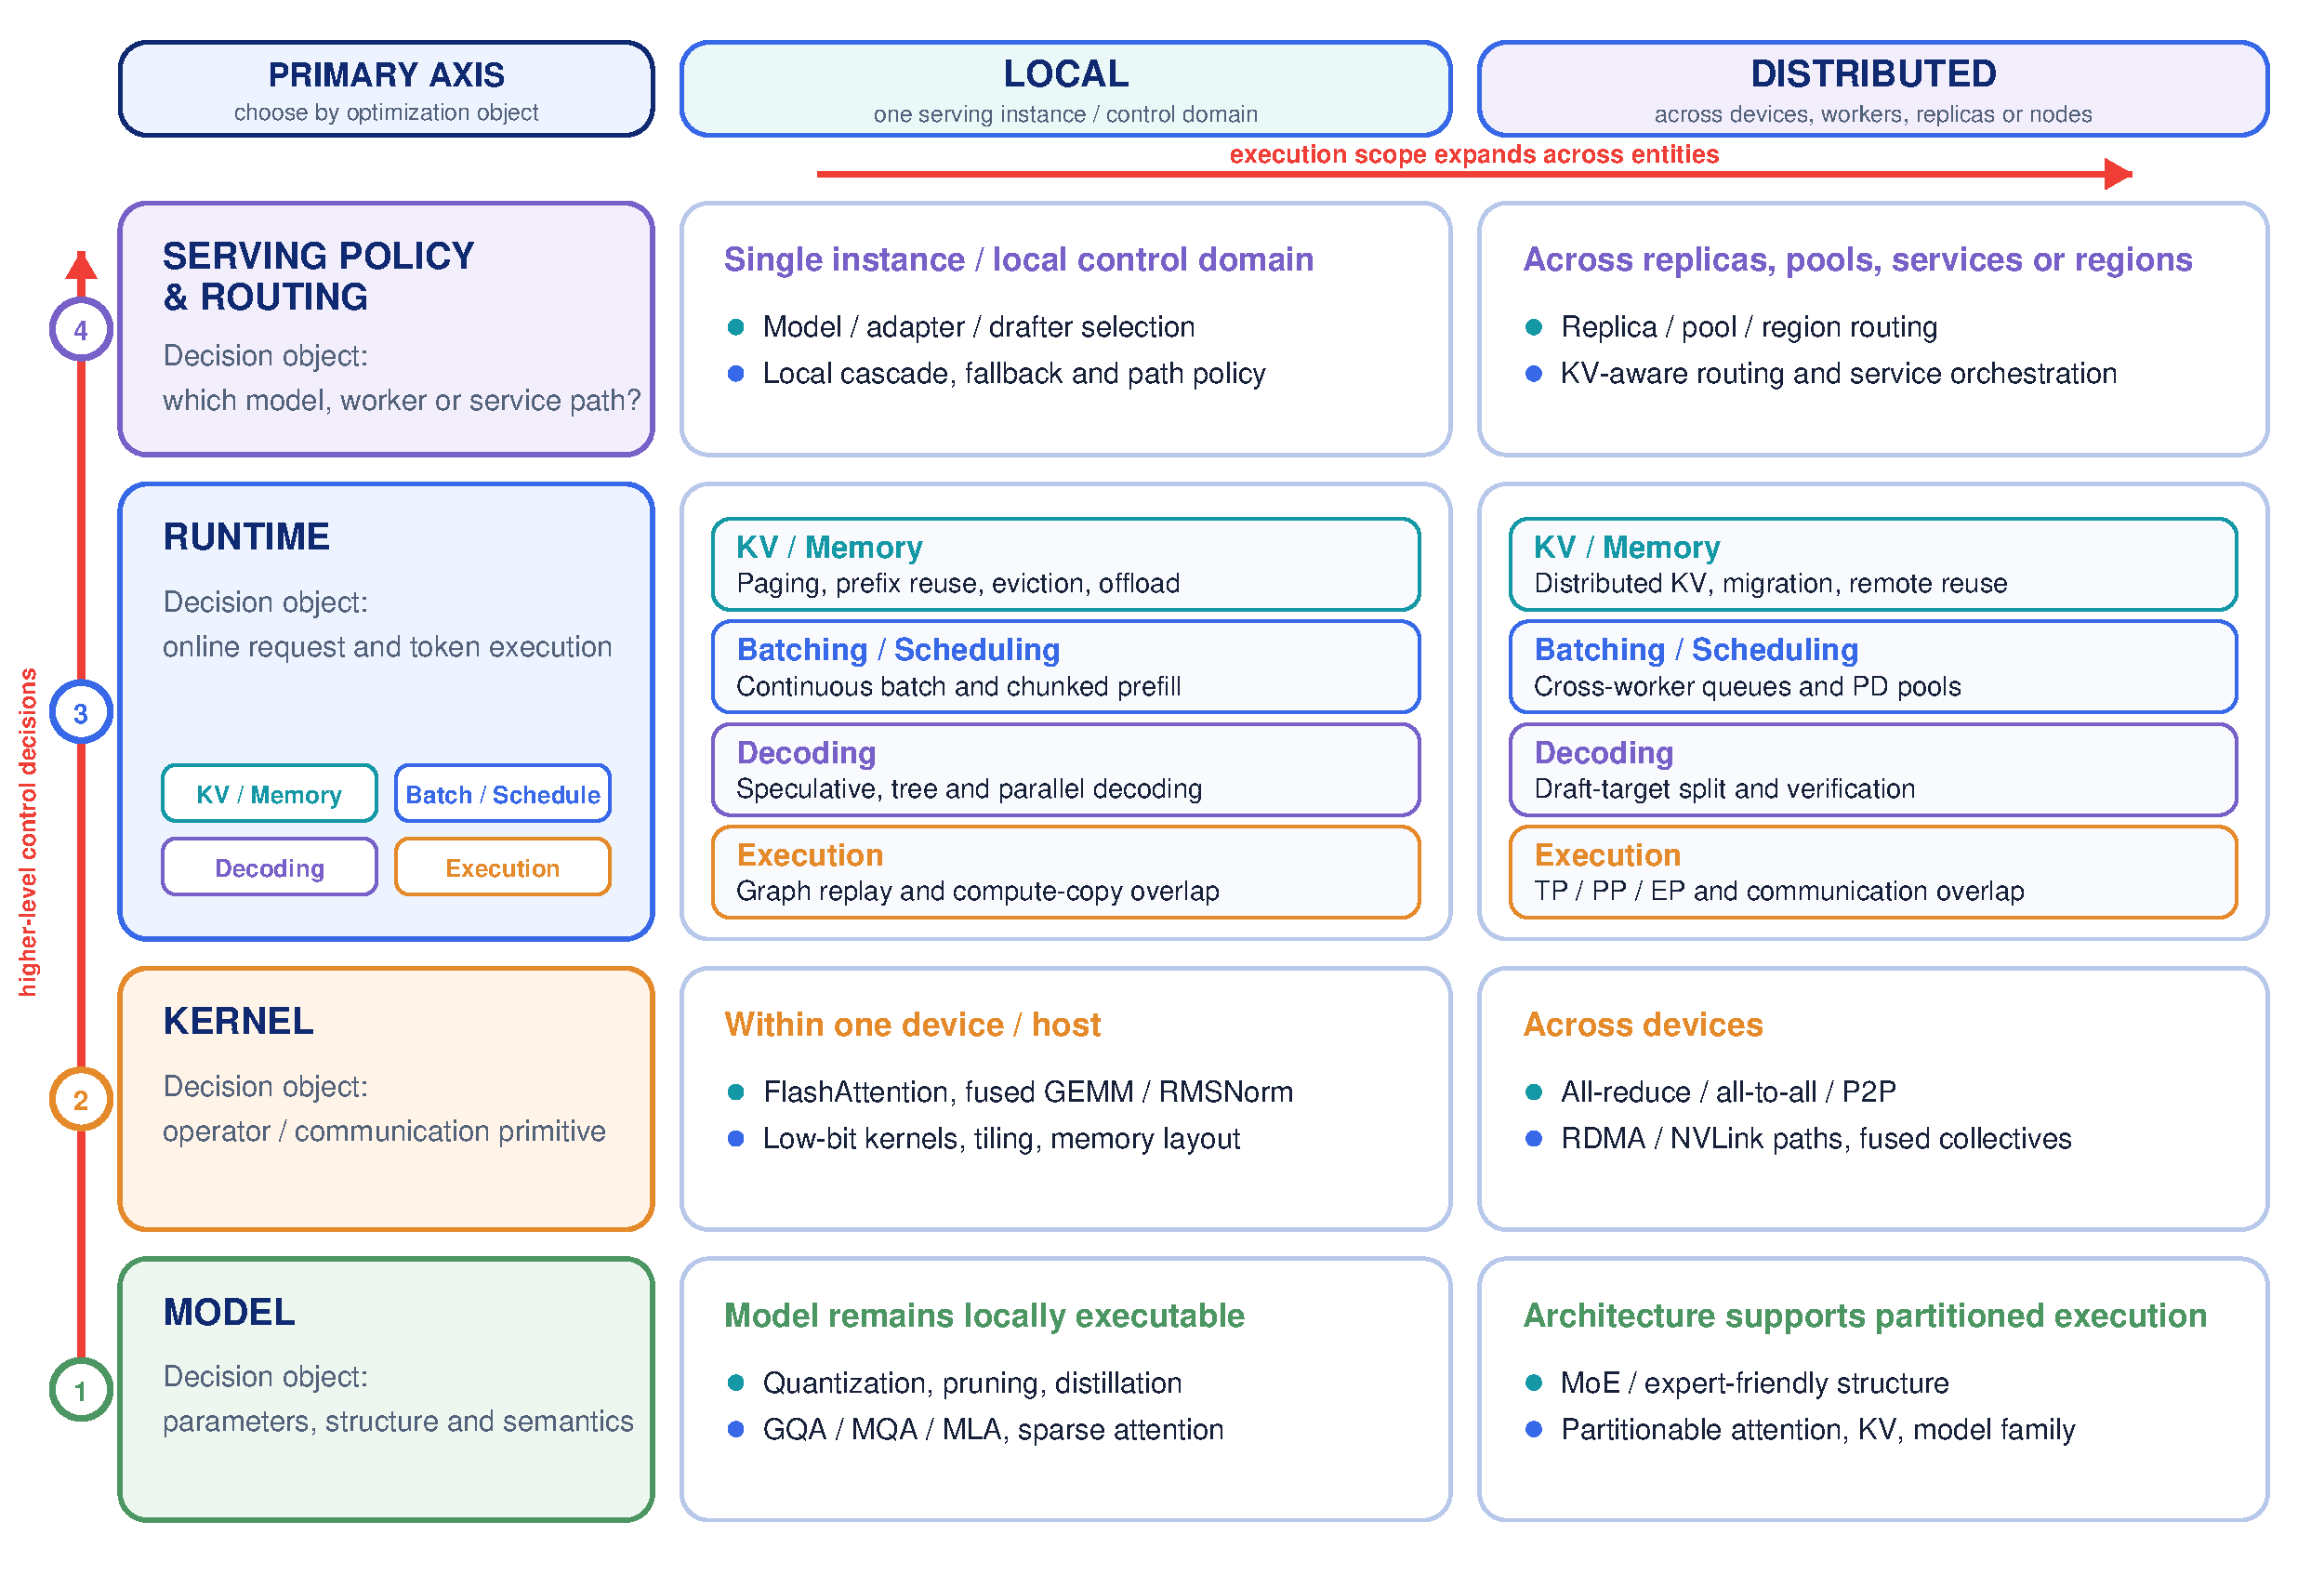
\includegraphics[width=\textwidth]{figures/ch2_layer_scope_taxonomy.pdf}
    \caption{\textbf{LLM 推理优化的“优化对象--执行范围”二维分类。}纵轴按照主要优化对象区分 Model、Kernel、Runtime 与 Serving Policy \& Routing 四个层级；横轴按照执行范围区分 Local 与 Distributed，表示方法从单实例或本地控制域扩展到跨设备、worker、replica、service 或 node 的协同。Runtime 层进一步包含 KV/Memory、Batching/Scheduling、Decoding 和 Execution 四类在线机制。}
    \label{fig:layer-scope-taxonomy}
\end{figure}

其中，Local 表示优化限制在单个 serving instance 或本地控制域内，可以包含 CPU 与 GPU/NPU、本地内存和存储之间的协同；Distributed 表示方法需要跨多个设备、worker、replica 或节点分配计算、请求、KV 状态或 activation。四类方法并不互斥，真实系统经常同时使用多层机制。因此，归类时主要判断三个问题：方法解决什么问题，直接改变的对象是什么，以及是否需要跨设备或跨节点协同。




\phantomsection
\subsubsection*{2.3.1 Model-Level Optimization}
\addcontentsline{toc}{subsubsection}{2.3.1 Model-Level Optimization}

Model-Level Optimization 直接改变模型参数、参数表示、结构设计或算法语义，以降低推理计算和存储开销。此类修改不依赖某个特定 serving engine，其优化对象包括参数量、权重表示、FLOPs、activation 计算量、attention 复杂度、KV 大小以及条件计算路径。

\textbf{Local scope：}常见方法包括权重量化、剪枝、蒸馏、低秩分解、权重共享、GQA/MQA/MLA、线性或稀疏 attention、状态空间模型、early exit、token pruning 和动态稀疏等，主要用于单实例或单设备上的模型压缩和结构简化。

\textbf{Distributed scope：}主要关注模型结构对跨设备执行的支持，例如适合 expert parallelism 的 MoE 结构、适合 tensor/context parallel 的 attention 或 KV 结构，以及便于按 layer、expert、context 或 activation 切分的模型设计。

CUDA Graph、算子融合和 TensorRT execution graph 等方法主要改变执行路径或部署图，分别归入 Runtime-Level 或 Kernel-Level；它们不会改变模型参数和数学语义。




\phantomsection
\subsubsection*{2.3.2 Kernel-Level Optimization}
\addcontentsline{toc}{subsubsection}{2.3.2 Kernel-Level Optimization}

Kernel-Level Optimization 在保持模型数学语义不变的条件下，优化张量算子或通信原语在硬件上的执行效率。主要对象包括 attention、GEMM、normalization、sampling 和 collective communication，目标是提高 GPU/NPU 利用率、减少 HBM 访问、增强片上缓存复用，并改善算子吞吐。

\textbf{Local scope：}典型方法包括 FlashAttention、FlashDecoding 和 paged attention kernel。其他方法还包括 MLP、RMSNorm 与 softmax 融合，低比特 GEMM，FP8、INT8 与 INT4 算子，硬件感知 tiling、内存布局优化和 GPU-side sampling。

\textbf{Distributed scope：}主要包括集合通信和点对点通信原语的实现优化，例如 all-reduce、all-gather、reduce-scatter、all-to-all、RDMA/NVLink 传输路径、通信融合、集合通信算法选择，以及 MoE expert dispatch/combine 原语。

需要区分的是，如果优化对象是 collective / P2P primitive 的实现路径，归为 Kernel-Level × Distributed；如果优化对象是通信与计算在 runtime pipeline 中的编排、重叠和调度，则归为 Runtime-Level × Distributed。




\phantomsection
\subsubsection*{2.3.3 Runtime-Level Optimization}
\addcontentsline{toc}{subsubsection}{2.3.3 Runtime-Level Optimization}

Runtime-Level Optimization 是现代 LLM serving 的主要系统优化层。它发生在请求进入 inference engine 之后，管理在线 token 执行、KV 状态、batch 组成、decode 循环和执行流水线。Runtime-Level 不改变模型语义，也不一定修改单个 kernel，而是决定请求到达后如何组织执行。本文将其进一步分为 KV / Memory、Batching / Scheduling、Decoding 和 Execution 四类运行时机制。

\begin{enumerate}
    \item \textbf{KV / Memory Runtime.} KV / Memory Runtime 关注 KV lifecycle、memory state 和 cache reuse。它的核心问题是：KV Cache 如何存储、复用、压缩、淘汰、迁移或远程访问。

    \textbf{Local scope：}主要包括 KV cache management、PagedAttention / memory paging、Prefix cache / RadixAttention、KV compression / quantization、KV eviction、KV offloading、cache persistence 和 runtime memory allocator 等机制。

    \textbf{Distributed scope：}问题进一步扩展为 distributed KV cache、KV transfer / migration、remote KV serving、multi-replica KV reuse、distributed prefix cache、KV-aware placement 和 cross-worker state synchronization。

    这一类优化的核心目标是降低 KV 显存占用、减少重复 prefill、提升 cache reuse，并在分布式场景下控制 KV 传输和状态迁移成本。

    \item \textbf{Batching / Scheduling Runtime.} Batching / Scheduling Runtime 关注请求和 token 在 inference engine 内如何组织执行。它回答的是：哪些请求何时执行，哪些 token 可以组成 batch，prefill 和 decode 如何交错，如何在 throughput、TTFT、TPOT、ITL、公平性和 SLA 之间做权衡。

    \textbf{Local scope：}典型机制包括 dynamic batching、continuous batching、iteration-level scheduling、chunked prefill、prefill/decode interleaving、engine-local admission control、priority / fair scheduling 和 deadline-aware scheduling。

    \textbf{Distributed scope：}调度对象会跨越 worker、replica 或资源池，因此需要 cross-worker scheduling、distributed continuous batching、prefill worker / decode worker scheduling、heterogeneous GPU scheduling、multi-replica queue coordination、distributed admission control 和 SLO-aware worker scheduling。

    这一类优化的核心目标是在动态请求负载下提高硬件利用率，同时控制排队时延和服务质量。

    \item \textbf{Decoding Runtime.} Decoding Runtime 关注在线 token generation procedure。它回答的是：输出 token 如何生成、验证、选择和接受。它不主要决定请求如何组 batch，也不主要决定计算如何 launch，而是改变 decode loop 的生成逻辑。

    \textbf{Local scope：}这类方法包括 speculative decoding、assisted decoding、parallel decoding、tree decoding、beam search optimization、n-gram speculation、prompt lookup decoding 和 serving-time multi-token prediction / verification。

    \textbf{Distributed scope：}Decoding Runtime 会涉及 distributed verification、draft / target execution split、multi-draft execution、batched verification across workers、draft model 与 target model 分布式协同，以及 speculative decoding 与 prefill/decode disaggregation 的结合。

    Speculative decoding 有时也被称为 decoding algorithm。本文将其主要归入 Runtime-Level，因为它改变的是服务阶段的 token 生成与验证过程，而不是原模型参数或主体结构。如果某种 multi-token prediction 方法新增训练 head 或修改模型结构，则还应同时标注其 Model-Level 属性。

    \item \textbf{Execution Runtime.} Execution Runtime 关注已经排定的计算如何提交、同步、重放和重叠执行。当前面的运行时已经决定请求集合、batch 组成和 decode 方式后，Execution Runtime 负责把算子、数据搬运和通信提交到硬件，并组织为流水线。

    \textbf{Local scope：}主要包括 CUDA Graph / HIP Graph replay、async execution、stream scheduling、CPU-GPU overlap、host-device communication hiding、compute / memory-copy overlap、runtime metadata / buffer reuse 和 GPU-side sampling execution path。

    \textbf{Distributed scope：}主要包括 tensor parallel runtime、pipeline parallel runtime、expert parallel runtime、context / sequence parallel runtime、prefill/decode disaggregation、distributed execution pipeline、communication-computation overlap scheduling 以及 activation / KV transfer orchestration。

    Execution Runtime 与 Kernel-Level 的边界在于：Kernel-Level 优化单个 operator 或 communication primitive 的实现；Execution Runtime 优化一组 operator、copy 和 communication 的 launch、同步、overlap 和流水化组织方式。
\end{enumerate}

\phantomsection
\subsubsection*{2.3.4 Serving Policy \& Routing-Level Optimization}
\addcontentsline{toc}{subsubsection}{2.3.4 Serving Policy \& Routing-Level Optimization}

Serving Policy \& Routing-Level Optimization 关注服务级控制决策。它不直接决定单个 engine 内部的 token 如何执行，而是选择请求使用哪个模型、adapter、replica、worker pool 或服务路径，并处理回退、级联和多服务编排。典型决策包括请求分配、模型或 adapter 选择、实例选择、服务路径选择，以及面向 SLO、成本和时延的路由策略。

\textbf{Local scope：}主要包括 local model selection、adapter / LoRA routing、local cascade serving、normal decoding 与 speculative decoding path selection、drafter selection、local/cloud fallback、budget-aware local inference 和 latency-aware local policy。

\textbf{Distributed scope：}进一步扩展为 replica routing、worker-pool routing、cluster load balancing、SLO-aware routing、cost-aware routing、region-aware routing、KV-aware routing、speculative serving orchestration、draft-target worker orchestration 和 multi-service graph orchestration。

Runtime-Level 和 Serving Policy \& Routing-Level 在真实系统中相互依赖，但主要决策对象不同。前者解决“请求进入某个 engine 后如何执行”，后者解决“请求交给哪个模型、worker、replica 或服务路径”。服务级决策通常需要读取队列长度、KV Cache 压力、batch 状态和请求距离 SLO 阈值的剩余时间。




\phantomsection
\subsection*{2.4 主流 LLM 推理框架及优化方式}
\addcontentsline{toc}{subsection}{2.4 主流 LLM 推理框架及优化方式}

LLM 推理框架把模型加载、算子执行、KV Cache 管理、请求调度和服务接口组合成可部署的推理系统。vLLM 以 PagedAttention 和 continuous batching 为基础，重点提高通用 GPU 服务器上的显存利用率与在线服务吞吐；TensorRT-LLM 面向 NVIDIA GPU，通过专用 kernel、低精度计算、in-flight batching 和多 GPU 并行提供高度优化的执行路径；SGLang 从结构化生成程序出发，将 RadixAttention、请求调度和分布式执行整合到同一运行时；LMDeploy/TurboMind 面向开源模型部署，提供模型转换与量化、persistent batching、blocked KV Cache 和多 GPU 执行等能力 \cite{kwon2023efficient,nvidia2026tensorrt,zheng2024sglang,lmdeploy2026documentation}。表~\ref{tab:framework-mechanism-mapping} 按主要优化对象和执行范围汇总这些框架的代表性机制；该表不覆盖各框架的全部功能。


\begin{table}[H]
    \centering
    \caption{\textbf{主流 LLM Inference Framework 代表性机制映射}}
    \label{tab:framework-mechanism-mapping}
    \renewcommand{\arraystretch}{1.45}
    \scriptsize
    \setlength{\tabcolsep}{4pt}
    \begin{tabularx}{\textwidth}{@{}>{\hsize=0.75\hsize\raggedright\arraybackslash}X >{\hsize=0.75\hsize\raggedright\arraybackslash}X >{\hsize=1.15\hsize\raggedright\arraybackslash}X >{\hsize=1.15\hsize\raggedright\arraybackslash}X >{\hsize=1.20\hsize\raggedright\arraybackslash}X@{}}
        \toprule
        \textbf{Framework} & \textbf{代表性方法 / 机制} & \textbf{解决的具体问题} & \textbf{优化方向分类层 \& Scope} & \textbf{具体方法说明} \\
        \midrule
        \frameworkcell{\textbf{vLLM}~\cite{kwon2023efficient}} & PagedAttention & KV Cache 动态分配和显存碎片问题 & Runtime / KV-Memory × Local & 通过分页式 KV 管理降低显存碎片，提高 KV Cache 利用率 \\
        \cmidrule(l){2-5}
         & Continuous batching & Decode 阶段请求动态进出，静态 batch 利用率低 & Runtime / Batching-Scheduling × Local & 在 decode iteration 动态加入和移除请求，提高高并发吞吐 \\
        \cmidrule(l){2-5}
         & Chunked prefill & 长 prompt prefill 阻塞 decode，影响 TTFT / ITL & Runtime / Batching-Scheduling × Local & 将长 prefill 拆分为 chunk，与 decode 交错执行 \\
        \cmidrule(l){2-5}
         & Prefix caching & 多请求共享前缀导致重复 prefill & Runtime / KV-Memory × Local/Distributed & 复用共享 prompt 或 prefix，减少重复 prefill 计算 \\
        \tabrowrule
        \frameworkcell{\textbf{TensorRT-LLM}~\cite{nvidia2026tensorrt}} & In-flight batching & 高并发请求长度不同，传统 batching 效率低 & Runtime / Batching-Scheduling × Local & 对不同阶段和长度的请求进行动态批处理 \\
        \cmidrule(l){2-5}
         & Paged KV Cache & KV Cache 分配、复用和显存管理问题 & Runtime / KV-Memory × Local & 通过 paged KV 管理改善 KV Cache 利用率 \\
        \cmidrule(l){2-5}
         & FP8 / INT8 / INT4 execution & 权重、activation 和算子执行成本高 & Model + Kernel × Local/Distributed & 通过低比特模型表示和低比特 kernel 降低显存和计算成本 \\
        \cmidrule(l){2-5}
         & Overlap scheduler & compute、copy、communication、prefill/decode 没有充分重叠 & Runtime / Execution × Local/Distributed & 将计算、通信和数据搬运流水线化，减少等待 \\
        \tabrowrule
        \frameworkcell{\textbf{SGLang}~\cite{zheng2024sglang}} & RadixAttention & 多轮、多分支请求存在大量共享前缀 & Runtime / KV-Memory × Local & 用 radix tree 组织 prefix cache，提高共享前缀复用 \\
        \cmidrule(l){2-5}
         & Zero-overhead CPU scheduler & 高并发场景下 CPU 调度开销影响吞吐 & Runtime / Batching-Scheduling × Local & 降低 CPU 侧调度和 metadata 管理开销 \\
        \cmidrule(l){2-5}
         & Prefill-decode disaggregation & Prefill 和 decode 资源特征不同，混部互相干扰 & Runtime / Execution × Distributed & 将 prefill 与 decode 分离到不同资源池，减少资源干扰 \\
        \cmidrule(l){2-5}
         & Multi-LoRA batching & 多 adapter 请求混合服务时 batch composition 复杂、吞吐下降 & Serving Policy \& Routing + Runtime/Scheduling × Local/Distributed & 将不同 LoRA / adapter 请求合并调度，提高多 LoRA serving 效率 \\
        \tabrowrule
        \frameworkcell{\textbf{Hugging Face TGI}~\cite{huggingface2026tgi}} & Continuous batching & incoming requests 动态变化，传统 batching 吞吐不足 & Runtime / Batching-Scheduling × Local & 动态合并请求，提高在线 serving 吞吐 \\
        \cmidrule(l){2-5}
         & Flash Attention & attention HBM traffic 高，operator throughput 受限 & Kernel × Local & 通过高效 attention kernel 降低显存访问并提升算子吞吐 \\
        \cmidrule(l){2-5}
         & Paged Attention & KV Cache / attention memory 管理效率不足 & Runtime / KV-Memory × Local & 通过 paged attention 改善 attention/KV memory 管理 \\
        \cmidrule(l){2-5}
         & Tensor parallelism & 单 GPU 容量或吞吐不足，需要跨 GPU 执行 & Runtime / Execution × Distributed & 将模型执行切分到多个 GPU，提高模型容量和吞吐 \\
        \tabrowrule
        \frameworkcell{\textbf{LMDeploy / TurboMind}~\cite{lmdeploy2026documentation}} & Persistent batching & 高并发请求动态调度，提高吞吐 & Runtime / Batching-Scheduling × Local & 通过持续批处理机制维持 batch 执行效率 \\
        \cmidrule(l){2-5}
         & Blocked KV Cache & KV Cache 显存管理和访问效率问题 & Runtime / KV-Memory × Local & 通过 block-based KV 管理改善显存利用率 \\
        \cmidrule(l){2-5}
         & Dynamic split \& fuse & 长 prompt 和 decode 混合执行效率低 & Runtime / Batching-Scheduling × Local & 动态拆分和融合 prefill / decode 任务，提高混合负载效率 \\
        \cmidrule(l){2-5}
         & Tensor parallelism & 大模型需要跨 GPU 执行 & Runtime / Execution × Distributed & 支持模型在多 GPU 上并行执行 \\
        \bottomrule
    \end{tabularx}
\end{table}

从主要部署对象看，上述框架目前仍以数据中心或服务器场景为主。其核心能力围绕单机多 GPU、多机多 GPU、高并发请求、稳定高速互联和统一加速器软件栈展开。具有兼容 GPU 或 NPU 的边缘服务器可以复用其中部分执行引擎，但这些框架本身通常不负责处理移动终端的功耗限制、端侧内存约束、间歇性链路、跨边缘节点状态放置和用户移动等问题。

边缘侧较有代表性的 LLM 推理框架包括 llama.cpp~\cite{llamacpp2026documentation} 和 MLC LLM~\cite{mlcllm2026documentation}。llama.cpp 使用轻量 C/C++ 运行时和 GGUF 模型格式，支持多种低比特量化、CPU/GPU 混合执行以及 Android 和 Apple 平台；MLC LLM 通过机器学习编译生成面向不同硬件后端的模型库，并以同一引擎支持 Web、iOS、Android、Python 和 REST 部署。这类框架的重点是让量化后的模型在单台手机、PC 或嵌入式设备上运行，其请求并发、跨节点 KV Cache 管理和全局调度能力仍弱于数据中心推理框架。

除单设备运行时外，已有部分研究围绕模型切分、异构资源调度和跨节点通信等问题，对多节点协同推理开展了方法设计与实验探索。总体来看，边缘侧单设备推理已具备较为成熟的软件实现，而多节点协同推理仍以面向特定问题的研究方案为主，尚未形成能够统一处理资源变化、链路波动、推理状态管理和用户移动的动态 CEC 服务框架。




\phantomsection
\subsection*{2.5 小结}
\addcontentsline{toc}{subsection}{2.5 小结}

本章首先介绍了 LLM inference 的基本执行机制，包括 prefill/decode、KV Cache、batching/scheduling 和主要性能指标。随后，从执行机制出发，总结了 LLM inference 的主要问题空间，包括计算复杂度与模型规模、KV Cache 与内存状态、请求动态性与调度、decode 串行性与生成加速，以及多实例、多 GPU 与服务级编排问题。


在已有 overview 和 survey 工作的基础上，本章采用“优化对象--执行范围”二维分类：按照方法直接改变的对象区分 Model、Kernel、Runtime、Serving Policy \& Routing，并按照是否跨设备或节点区分 Local 与 Distributed。Runtime 层进一步细分为 KV / Memory、Batching / Scheduling、Decoding 和 Execution 四类机制。该分类可同时说明一个方法改动了什么，以及它在单实例内执行还是需要分布式协同。


最后，本章通过主流推理框架的代表性机制映射说明，实际系统通常会组合模型表示、kernel、KV 管理、batching/scheduling、执行运行时和服务策略等多层机制。现有通用服务框架主要面向数据中心，边缘侧单设备运行时已经具备工程可用性，而多节点协同服务仍以研究原型为主。该分类框架将用于后续分析 CEC 场景下的模型部署、请求调度、KV 状态迁移和服务路径选择。
